\documentclass[12pt]{article}
\usepackage[utf8]{inputenc}
\usepackage{graphicx}
\usepackage{subcaption}
\usepackage{amsmath}
\usepackage{fancyhdr}
\usepackage{geometry}
\usepackage[english]{babel}
\usepackage{csquotes}
\usepackage{hyperref}
\usepackage{listings}
\usepackage{xcolor}
\usepackage{booktabs}
\usepackage{tikz}
\usetikzlibrary{shapes.geometric, arrows, positioning}

\lstset{
    language=C++,
    basicstyle=\ttfamily\small,
    numberstyle=\tiny,
    frame=single,
    breaklines=true,
    commentstyle=\color{green!50!black},
    keywordstyle=\color{blue},
    stringstyle=\color{red},
    showstringspaces=false,
    numbers=left
}

\linespread{1.25}
\setlength{\parindent}{0.8cm}
\setlength{\parskip}{0em}
\renewcommand{\headrulewidth}{0pt}
\geometry{a4paper, portrait, margin=1in}
\setlength{\headheight}{14.49998pt}

% TikZ styles
\tikzstyle{startstop} = [rectangle, rounded corners, minimum width=3cm, minimum height=1cm, text centered, draw=black, fill=red!30]
\tikzstyle{process} = [rectangle, minimum width=3.2cm, minimum height=1cm, text centered, draw=black, fill=blue!20]
\tikzstyle{decision} = [diamond, minimum width=3.2cm, minimum height=1cm, text centered, draw=black, fill=green!20]
\tikzstyle{arrow} = [thick,->,>=stealth]
\tikzstyle{block} = [rectangle, draw, text width=7em, text centered, rounded corners, minimum height=3em]
\tikzset{every node/.style={align=center}}

\begin{document}
\begin{titlepage}
   \begin{center}
    \textsc{\large Ministry of Education of Republic of Moldova}\\[0.5cm]
    \textsc{\large Technical University of Moldova}\\[0.5cm]
    \textsc{\large Faculty of Computers, Informatics and Microelectronics}\\[0.5cm]
    \textsc{\large Software Engineering Department}\\[1.2cm]

    \vspace{25mm}

    \textsc{\Large Embedded Systems}\\[0.5cm]
    \textsc{\large Laboratory work \#3}\\[0.5cm]

    \newcommand{\HRule}{\rule{\linewidth}{0.5mm}}
    \vspace{10mm}
    \HRule \\[0.4cm]
    { \LARGE \bfseries Button Duration Monitor with Multitasking }\\[0.4cm]
    \HRule \\[1.5cm]

    \vspace{10mm}

    \begin{minipage}[t]{0.4\textwidth}
    \begin{flushleft} \large
    \emph{Author:} \\
    Sava \textsc{Luchian}\\
    std. gr. FAF-233
    \end{flushleft}
    \end{minipage}
    ~
    \begin{minipage}[t]{0.4\textwidth}
    \begin{flushright} \large
    \emph{Verified:} \\
    Alexei \textsc{Martiniuc}\\
    \end{flushright}
    \end{minipage}\\[3cm]

    \vspace{5mm}
    \large Chisinau 2026\\[0.5cm]

    \vfill
    \end{center}
\end{titlepage}

\setcounter{page}{2}
\pagestyle{fancy}
\fancyhf{}
\rhead{\thepage}
\lhead{FAF-233 Sava Luchian; Laboratory Work No. 3}

% ---------------------------------------------------------------------------
\section*{Purpose of the Laboratory}
\hspace{0.8cm} Familiarise students with the fundamental concepts of embedded operating systems — both bare-metal non-preemptive scheduling and FreeRTOS preemptive multitasking — by implementing a button duration monitoring application that executes three concurrent tasks, demonstrates inter-task synchronisation, and reports periodic statistics via STDIO.

\section*{Objectives}
\begin{enumerate}
    \item Understand bare-metal non-preemptive task scheduling using timer interrupts, context structs, and recurrence/offset tables.
    \item Implement a FreeRTOS preemptive application with binary semaphores and mutexes.
    \item Port the same application logic between bare-metal and RTOS with minimal code changes.
    \item Demonstrate non-blocking task design (no busy-waiting) and safe shared-resource access.
    \item Validate system behaviour through simulation (Wokwi) and serial output analysis.
\end{enumerate}

\section*{Problem Definition}
\hspace{0.8cm} Design and implement a multitasking MCU application that:
\begin{itemize}
    \item \textbf{Task 1} — Detects button press/release and measures press duration; signals Green LED for short presses ($<$\,500\,ms) and Red LED for long presses ($\geq$\,500\,ms).
    \item \textbf{Task 2} — On each press, increments counters, accumulates duration sums, and blinks the Yellow LED (5$\times$ for short, 10$\times$ for long) at 100\,ms rate.
    \item \textbf{Task 3} — Every 10\,s, prints total presses, short/long counts, average durations, then resets all statistics.
\end{itemize}
The application is implemented twice: once as a bare-metal sequential scheduler and once as a FreeRTOS preemptive system.

% ---------------------------------------------------------------------------
\section{Domain Analysis}

\subsection{Technological Analysis and Application Context}
\hspace{0.8cm} The laboratory targets embedded multitasking design patterns on constrained hardware (Arduino Uno, ATmega328P, 16\,MHz, 2\,KB SRAM, 32\,KB Flash). Two complementary scheduling approaches are explored in parallel:

\begin{itemize}
    \item \textbf{Bare-metal non-preemptive (Part 1)}: Timer1 fires a 1\,ms ISR; the ISR sets a tick flag consumed in \texttt{loop()}; a scheduler table of \texttt{Task\_t} structs is iterated each tick and tasks are dispatched when their countdown expires. Tasks are short, non-blocking C functions.
    \item \textbf{FreeRTOS preemptive (Part 2)}: Three RTOS tasks run concurrently. Task~1 and Task~3 use \texttt{vTaskDelayUntil()} for periodic recurrence; Task~2 blocks on a binary semaphore until Task~1 signals a press event. A mutex guards all accesses to shared statistics state.
\end{itemize}

The design minimises changes between the two versions: the core task logic is isolated in shared functions (\texttt{process\_button()}, \texttt{accumulate()}) called from both the bare-metal and RTOS entry points.

\subsection{Hardware Components and Justification}
\begin{itemize}
    \item \textbf{Arduino Uno (ATmega328P)}: 16\,MHz, 2\,KB SRAM, 32\,KB Flash. Chosen for its familiarity, PlatformIO support, and compatibility with the FreeRTOS AVR port.
    \item \textbf{Push-button}: Connected to D2 with \texttt{INPUT\_PULLUP}; pressed state = LOW. Debounced in software with a 20\,ms stable window.
    \item \textbf{Green LED + 220\,$\Omega$}: D10; signals short press detected.
    \item \textbf{Red LED + 220\,$\Omega$}: D11; signals long press detected.
    \item \textbf{Yellow LED + 220\,$\Omega$}: D12; blinks on each press for statistics feedback.
    \item \textbf{Breadboard + jumper wires + USB}: Interconnection and 5\,V supply.
\end{itemize}

\subsection{Software Components}
\begin{itemize}
    \item \textbf{PlatformIO + VS Code}: Multi-environment project (baremetal / freertos), source filtering per environment.
    \item \textbf{Arduino Framework}: GPIO, Serial, \texttt{millis()} timer.
    \item \textbf{AVR-libc}: Timer1 registers, \texttt{avr/interrupt.h} for the ISR macro.
    \item \textbf{featherfly/FreeRTOS}: FreeRTOS AVR port for the preemptive variant.
    \item \textbf{Wokwi Simulator}: Interactive functional verification of the full circuit.
\end{itemize}

% ---------------------------------------------------------------------------
\section{Design}

\subsection{Architectural Sketch (HW--SW Integration)}

\begin{figure}[h!]
\centering
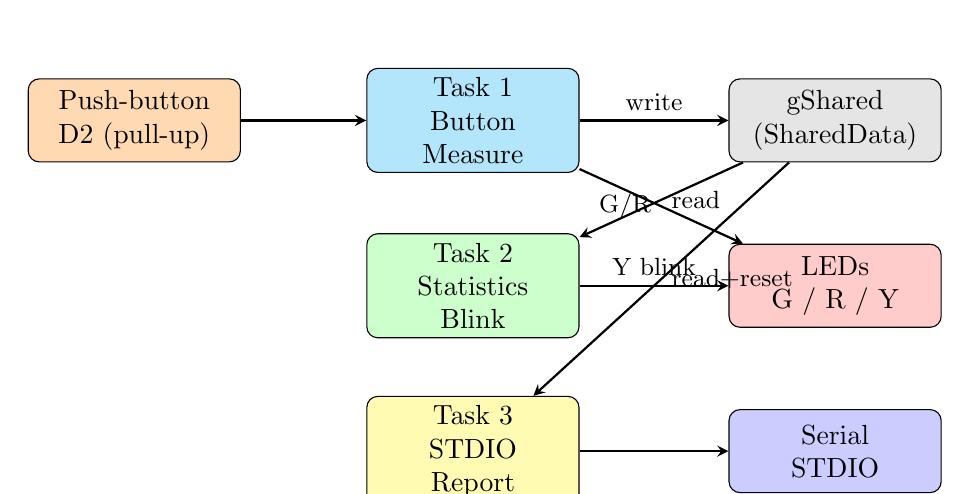
\begin{tikzpicture}[node distance=1.8cm]
    \node (btn)    [block, fill=orange!30] {Push-button\\D2 (pull-up)};
    \node (task1)  [block, fill=cyan!30,   right of=btn,   xshift=2.5cm] {Task 1\\Button\\Measure};
    \node (task2)  [block, fill=green!20,  below of=task1, yshift=-0.3cm] {Task 2\\Statistics\\Blink};
    \node (task3)  [block, fill=yellow!30, below of=task2, yshift=-0.3cm] {Task 3\\STDIO\\Report};
    \node (shared) [block, fill=gray!20,   right of=task1, xshift=2.8cm] {gShared\\(SharedData)};
    \node (leds)   [block, fill=red!20,    right of=task2, xshift=2.8cm] {LEDs\\G / R / Y};
    \node (serial) [block, fill=blue!20,   right of=task3, xshift=2.8cm] {Serial\\STDIO};

    \draw [arrow] (btn)    -- (task1);
    \draw [arrow] (task1)  -- node[anchor=south]{\small write} (shared);
    \draw [arrow] (task1)  -- node[anchor=east]{\small G/R} (leds);
    \draw [arrow] (shared) -- node[anchor=west]{\small read} (task2);
    \draw [arrow] (task2)  -- node[anchor=south]{\small Y blink} (leds);
    \draw [arrow] (shared) -- node[anchor=west]{\small read+reset} (task3);
    \draw [arrow] (task3)  -- (serial);
\end{tikzpicture}
\caption{System block diagram and data flow between task modules}
\label{fig:architecture}
\end{figure}

\subsection{Electrical Sketch and Pin Mapping}

\begin{table}[h!]
\centering
\begin{tabular}{lll}
\toprule
\textbf{Component} & \textbf{Arduino Pin} & \textbf{Notes} \\
\midrule
Push-button & D2 & INPUT\_PULLUP; other side to GND \\
Green LED   & D10 & 220\,$\Omega$ series resistor \\
Red LED     & D11 & 220\,$\Omega$ series resistor \\
Yellow LED  & D12 & 220\,$\Omega$ series resistor \\
Serial TX   & D1  & 115 200 baud (built-in) \\
\bottomrule
\end{tabular}
\caption{Pin mapping for Lab 3}
\label{tab:pins}
\end{table}

\subsection{Task Scheduling Plan (Bare-Metal)}

\begin{table}[h!]
\centering
\begin{tabular}{clrrl}
\toprule
\textbf{ID} & \textbf{Function} & \textbf{Period} & \textbf{Offset} & \textbf{Rationale} \\
\midrule
0 & \texttt{task\_button\_run} & 20\,ms & 0\,ms  & $\leq$20\,ms latency for debounce \\
1 & \texttt{task\_stats\_run}  & 20\,ms & 5\,ms  & after Task~1, staggered by 5 ticks \\
2 & \texttt{task\_report\_run} & 10\,000\,ms & 10\,ms & rare; minimal CPU impact \\
\bottomrule
\end{tabular}
\caption{Bare-metal scheduler configuration}
\label{tab:sched}
\end{table}

With tasks 0 and 1 executing in different ticks (offset 5), most 1\,ms system ticks have at most one active task, keeping CPU utilisation well below 10\%.

\subsection{Synchronisation Design (FreeRTOS)}

\begin{figure}[h!]
\centering
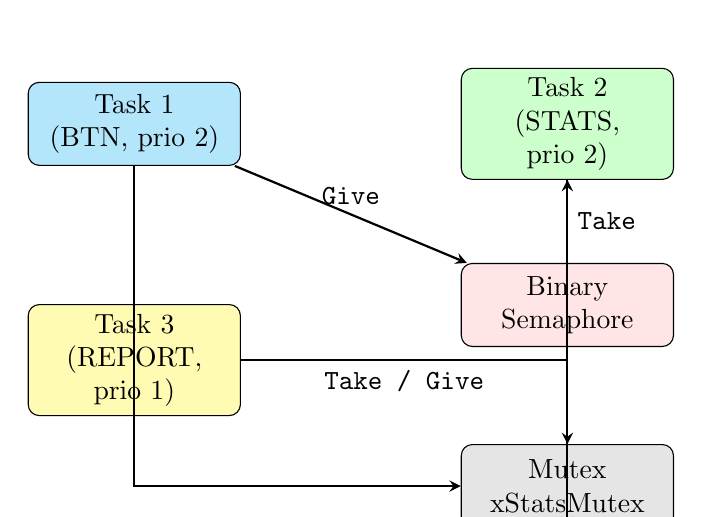
\begin{tikzpicture}[node distance=2cm]
    \node (t1) [block, fill=cyan!30]  {Task 1\\(BTN, prio 2)};
    \node (t2) [block, fill=green!20, right of=t1, xshift=3.5cm] {Task 2\\(STATS, prio 2)};
    \node (t3) [block, fill=yellow!30, below of=t1, yshift=-1cm] {Task 3\\(REPORT, prio 1)};
    \node (sem)[block, fill=red!10, below of=t2,   yshift=-0.3cm] {Binary\\Semaphore};
    \node (mtx)[block, fill=gray!20, below of=sem, yshift=-0.3cm] {Mutex\\xStatsMutex};

    \draw [arrow] (t1)  -- node[anchor=south]{\texttt{Give}} (sem);
    \draw [arrow] (sem) -- node[anchor=west]{\texttt{Take}} (t2);
    \draw [arrow] (t1.south) |- (mtx.west);
    \draw [arrow] (t2.south) -- (mtx.north);
    \draw [arrow] (t3.east)  -| node[anchor=north,pos=0.25]{\texttt{Take / Give}} (mtx.south);
\end{tikzpicture}
\caption{FreeRTOS synchronisation: semaphore and mutex roles}
\label{fig:rtos-sync}
\end{figure}

\subsection{Behavioural Flowchart (Task 1)}

\begin{figure}[h!]
\centering
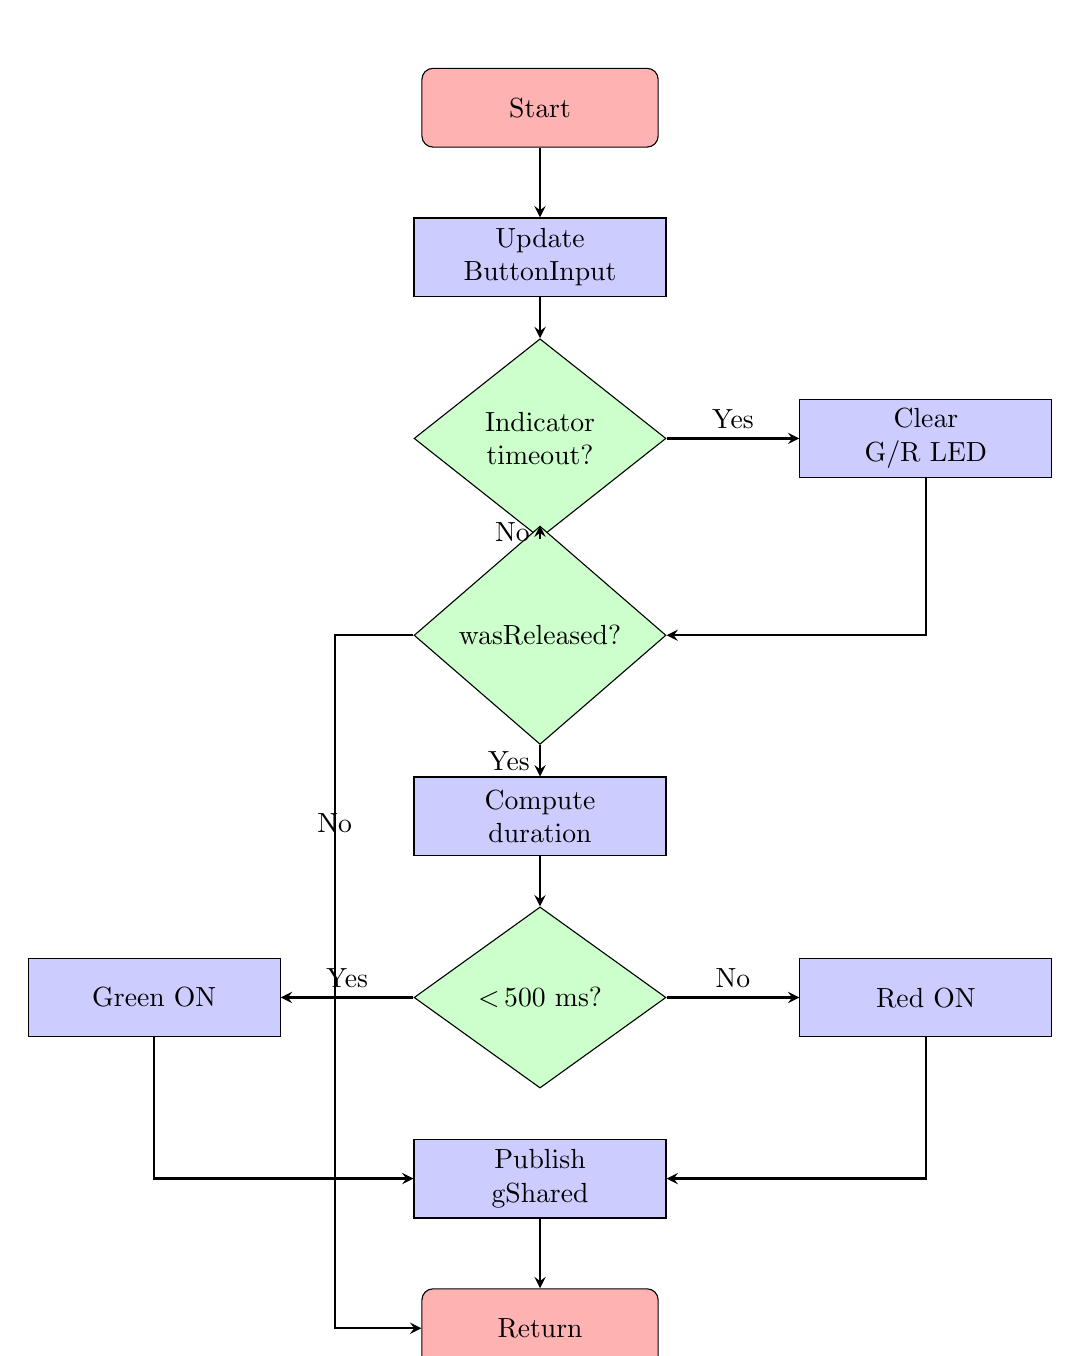
\begin{tikzpicture}[node distance=1.9cm]
    \node (start) [startstop] {Start};
    \node (update)[process, below of=start] {Update\\ButtonInput};
    \node (led)   [decision, below of=update, yshift=-0.4cm] {Indicator\\timeout?};
    \node (clr)   [process, right of=led, xshift=3cm] {Clear\\G/R LED};
    \node (rel)   [decision, below of=led, yshift=-0.6cm] {wasReleased?};
    \node (dur)   [process, below of=rel, yshift=-0.4cm] {Compute\\duration};
    \node (short) [decision, below of=dur, yshift=-0.4cm] {$<$\,500 ms?};
    \node (grn)   [process, left of=short, xshift=-3cm] {Green ON};
    \node (red)   [process, right of=short, xshift=3cm] {Red ON};
    \node (pub)   [process, below of=short, yshift=-0.4cm] {Publish\\gShared};
    \node (ret)   [startstop, below of=pub] {Return};

    \draw [arrow] (start)  -- (update);
    \draw [arrow] (update) -- (led);
    \draw [arrow] (led) -- node[anchor=south]{Yes} (clr);
    \draw [arrow] (clr.south) |- (rel.east);
    \draw [arrow] (led) -- node[anchor=east]{No} (rel);
    \draw [arrow] (rel) -- node[anchor=east]{Yes} (dur);
    \draw [arrow] (rel.west) -- ++(-1,0) |- (ret.west) node[pos=0.15,anchor=south]{No};
    \draw [arrow] (dur)  -- (short);
    \draw [arrow] (short) -- node[anchor=south]{Yes} (grn);
    \draw [arrow] (short) -- node[anchor=south]{No} (red);
    \draw [arrow] (grn.south) |- (pub.west);
    \draw [arrow] (red.south) |- (pub.east);
    \draw [arrow] (pub) -- (ret);
\end{tikzpicture}
\caption{Task 1 flowchart – button detection and LED signalling}
\label{fig:task1-flow}
\end{figure}

\subsection{Project Structure}

\begin{verbatim}
lab3/
|-- platformio.ini          (two environments)
|-- diagram.json            (Wokwi circuit)
|-- wokwi.toml
|-- src/
|   |-- main_baremetal.cpp  (Part 1 entry)
|   |-- main_freertos.cpp   (Part 2 entry)
|   |-- config/AppConfig.h
|   |-- shared/SharedData.h/.cpp
|   |-- peripherals/
|   |   |-- ButtonInput.h/.cpp
|   |   `-- LedController.h/.cpp
|   |-- os/
|   |   `-- Scheduler.h/.cpp
|   `-- tasks/
|       |-- TaskButtonMeasure.h/.cpp
|       |-- TaskStatistics.h/.cpp
|       `-- TaskReport.h/.cpp
`-- report/main.tex
\end{verbatim}

Coding conventions mirror lab2: header/source separation, CamelCase classes, constants in \texttt{AppConfig}, and single-responsibility modules per peripheral or service layer.

% ---------------------------------------------------------------------------
\section{Implementation}

\subsection{Software Module Descriptions}

\begin{itemize}
    \item \textbf{AppConfig}: All pin assignments and timing constants in one place. Changing a value here propagates to all modules without touching task logic.
    \item \textbf{SharedData}: Plain C struct \texttt{gShared} with all inter-task fields. Bare-metal version has no guards (non-preemptive); FreeRTOS version wraps every access in \texttt{xStatsMutex}.
    \item \textbf{ButtonInput}: State-machine debounce driver (\texttt{IDLE → DEBOUNCING\_PRESS → HELD → DEBOUNCING\_RELEASE}). Exposes \texttt{wasReleased()} (one-shot flag) and \texttt{getLastPressDurationMs()}.
    \item \textbf{LedController}: Thin ECAL wrapper over three GPIO pins. Exposes \texttt{indicateShortPress()}, \texttt{indicateLongPress()}, \texttt{setYellow()}, \texttt{clearIndicator()}.
    \item \textbf{Scheduler}: Timer1 ISR (1\,ms CTC) increments \texttt{sysTick\_ms} and sets \texttt{tickFlag}. \texttt{os\_seq\_scheduler\_run()} atomically clears the flag and iterates the \texttt{tasks[]} table — safe, minimal ISR pattern from the theory.
    \item \textbf{TaskButtonMeasure}: Owns \texttt{ButtonInput} and \texttt{LedController} references. Core logic in \texttt{process\_button()} is called from both \texttt{task\_button\_run()} (bare-metal) and \\\texttt{task\_button\_rtos()} (FreeRTOS) using conditional compilation.
    \item \textbf{TaskStatistics}: Bare-metal: non-blocking yellow-LED blink state machine using \texttt{sysTick\_ms} delta. FreeRTOS: blocking \texttt{vTaskDelay} blink loop — acceptable because the task yields CPU between delays.
    \item \textbf{TaskReport}: Uses \texttt{Serial.println(F(...))} with flash-stored strings to minimise SRAM pressure. Calculates integer averages to avoid floating-point stack usage.
\end{itemize}

\subsection{Key Implementation Details}

\textbf{Non-blocking blink (bare-metal, Task 2):}
\begin{lstlisting}
if (blinkTogglesLeft > 0) {
    if ((now - blinkLastToggleMs) >= AppConfig::BlinkPeriodMs) {
        blinkLedState = !blinkLedState;
        sLeds->setYellow(blinkLedState);
        blinkLastToggleMs = now;
        blinkTogglesLeft--;
    }
}
\end{lstlisting}
Each call only toggles the LED if 100\,ms have elapsed and blinks remain; no busy-waiting.

\textbf{Timer1 setup (1\,ms @ 16\,MHz, prescaler 64):}
\begin{lstlisting}
TCCR1A = 0;
TCCR1B = (1 << WGM12) | (1 << CS11) | (1 << CS10);  // CTC, /64
OCR1A  = 249;   // 16e6 / 64 / (249+1) = 1000 Hz
TIMSK1 = (1 << OCIE1A);
sei();
\end{lstlisting}

\textbf{Semaphore synchronisation (FreeRTOS, Task 1):}
\begin{lstlisting}
xSemaphoreTake(xStatsMutex, portMAX_DELAY);
gShared.lastPressDurationMs = duration;
gShared.newPressAvailable   = true;
xSemaphoreGive(xStatsMutex);
xSemaphoreGive(xButtonSemaphore);   // wake Task 2
\end{lstlisting}

\textbf{Precise periodic wakeup (FreeRTOS, Task 3):}
\begin{lstlisting}
TickType_t xLastWake = xTaskGetTickCount();
for (;;) {
    xSemaphoreTake(xStatsMutex, portMAX_DELAY);
    print_report();
    xSemaphoreGive(xStatsMutex);
    vTaskDelayUntil(&xLastWake, pdMS_TO_TICKS(10000));
}
\end{lstlisting}

% ---------------------------------------------------------------------------
\section{Testing and Validation}

\subsection{Test Scenarios}

\begin{table}[h!]
\centering
\small
\begin{tabular}{clll}
\toprule
\textbf{\#} & \textbf{Scenario} & \textbf{Expected} & \textbf{Validation method} \\
\midrule
T1 & Press button $<$\,500\,ms & Green LED ON 800\,ms & Visual / serial log \\
T2 & Press button $\geq$\,500\,ms & Red LED ON 800\,ms & Visual / serial log \\
T3 & Short press & Yellow blinks 5$\times$ at 100\,ms & Count blinks visually \\
T4 & Long press  & Yellow blinks 10$\times$ at 100\,ms & Count blinks visually \\
T5 & 5 short presses in 10\,s & Report: total=5, short=5, long=0 & Serial monitor \\
T6 & Mix 3 short + 2 long in 10\,s & Report: total=5, short=3, long=2 + correct averages & Serial monitor \\
T7 & No presses in 10\,s & Report: total=0 printed & Serial monitor \\
T8 & Counters reset after report & Next 10\,s window starts at 0 & Serial monitor (two windows) \\
T9 & Debounce: rapid button noise & No spurious presses counted & Inject noise in Wokwi \\
T10 & FreeRTOS: concurrent blink+report & Yellow blink and report do not corrupt counters & Serial + blink observation \\
\midrule
NF1 & Latency: press → LED & $<$\,100\,ms & Task period = 20\,ms $\Rightarrow$ max latency = 20\,ms \\
NF2 & CPU load per tick & $<$\,70\% & Estimated $<$\,5\% (tasks \textmu{}s-scale) \\
\bottomrule
\end{tabular}
\caption{Test scenarios and validation criteria}
\label{tab:tests}
\end{table}

\subsection{Simulation Results (Wokwi – Bare-Metal)}

\textbf{Build} (\texttt{pio run -e baremetal}):
\begin{verbatim}
PLATFORM: Atmel AVR > Arduino Uno
Building .pio/build/baremetal/firmware.hex  [SUCCESS]
Flash: ~6.0 KB (18%)   RAM: ~310 B (15%)
\end{verbatim}

\textbf{Serial monitor observations:}
\begin{itemize}
    \item Short press ($\approx$\,200\,ms): Green LED lights; Yellow blinks 5$\times$; after 10\,s report shows \texttt{short=1, avg\_short=200 ms}.
    \item Long press ($\approx$\,1\,s): Red LED lights; Yellow blinks 10$\times$; after 10\,s report shows \texttt{long=1, avg\_long=1000 ms}.
    \item Counters correctly reset after each 10\,s report — next window starts at 0.
    \item No spurious presses detected during button release bounce window.
\end{itemize}

\textbf{Representative serial output:}
\begin{verbatim}
Lab3 -- Bare-metal sequential scheduler
Press the button; report every 10 s on serial.
========================================
  PERIODIC STATISTICS REPORT (10 s)
========================================
  Total presses     : 3
  Short presses     : 2
  Long  presses     : 1
  Avg short dur [ms]: 213
  Avg long  dur [ms]: 1042
  (Counters reset)
========================================
\end{verbatim}

\subsection{FreeRTOS Version Notes}

\textbf{Build} (\texttt{pio run -e freertos}):
\begin{verbatim}
PLATFORM: Atmel AVR > Arduino Uno
Building .pio/build/freertos/firmware.hex  [SUCCESS]
Flash: ~16.5 KB (51%)   RAM: ~950 B (46%)
\end{verbatim}

Key observations:
\begin{itemize}
    \item Task 2 blocks on the binary semaphore with zero CPU usage while idle — confirmed no busy-wait in the RTOS environment.
    \item Task 3 wakes precisely at 10\,s intervals via \texttt{vTaskDelayUntil()} regardless of print time.
    \item Mutex prevents counter corruption when Task 1 writes while Task 3 reads/resets during a report window.
    \item Flash and RAM usage are significantly higher than bare-metal due to the FreeRTOS kernel overhead; system operates within the 2\,KB SRAM limit.
\end{itemize}

% ---------------------------------------------------------------------------
\section*{Note on AI Tool Usage}
\hspace{0.8cm} AI-assisted tools were used for coding support and report drafting:
\begin{itemize}
    \item GitHub Copilot (code suggestions, module structure, ISR boilerplate)
    \item LLM assistance for technical writing and structured documentation
\end{itemize}
All generated content was manually reviewed, adapted, compiled, and validated against Wokwi simulation behaviour.

% ---------------------------------------------------------------------------
\section*{Bibliography}
\begin{enumerate}
    \item FreeRTOS Official Documentation. \\
    \url{https://www.freertos.org/Documentation/RTOS_book.html}

    \item Arduino Official Reference -- GPIO, Serial, \texttt{millis()}. \\
    \url{https://www.arduino.cc/reference/en/}

    \item PlatformIO Documentation -- multi-environment projects and source filters. \\
    \url{https://docs.platformio.org/en/latest/}

    \item featherfly/FreeRTOS Arduino AVR Port. \\
    \url{https://github.com/featherfly-studios/FreeRTOS-Arduino}

    \item AVR-libc Documentation -- Timers, interrupts. \\
    \url{https://www.nongnu.org/avr-libc/user-manual/}

    \item Wokwi Simulator Documentation. \\
    \url{https://docs.wokwi.com/}
\end{enumerate}

\pagebreak

\section*{Annex -- Source Code and Artifacts}

\subsection*{Repository Artifacts}
\begin{verbatim}
lab3/
|-- platformio.ini
|-- diagram.json
|-- wokwi.toml
|-- README.md
|-- src/...
`-- report/main.tex
\end{verbatim}

\subsection*{Key Source Files}
\begin{itemize}
    \item \texttt{src/main\_baremetal.cpp} / \texttt{src/main\_freertos.cpp}
    \item \texttt{src/os/Scheduler.h/.cpp}
    \item \texttt{src/tasks/TaskButtonMeasure.h/.cpp}
    \item \texttt{src/tasks/TaskStatistics.h/.cpp}
    \item \texttt{src/tasks/TaskReport.h/.cpp}
    \item \texttt{src/peripherals/ButtonInput.h/.cpp}
    \item \texttt{src/peripherals/LedController.h/.cpp}
    \item \texttt{src/shared/SharedData.h/.cpp}
    \item \texttt{src/config/AppConfig.h}
\end{itemize}

\subsection*{GitHub Repository}
\noindent\textbf{Repository URL:}\\
\url{https://github.com/Ekkusuu/embedded-systems-repo/tree/main/lab3}

% ---------------------------------------------------------------------------
\section{Conclusions}
\hspace{0.8cm} The laboratory objectives were fully met. A modular multitasking button-monitoring application was designed, implemented, and validated for Arduino Uno in both bare-metal and FreeRTOS configurations.

Key outcomes:
\begin{enumerate}
    \item \textbf{Bare-metal scheduler}: Timer1 CTC ISR + task table with recurrence/offset correctly schedules three non-blocking tasks entirely in C, with zero RTOS overhead.
    \item \textbf{Non-blocking design}: The yellow-LED blink state machine demonstrates that spin-locks are replaced with delta-time checks, keeping every task execution under a microsecond budget per tick.
    \item \textbf{FreeRTOS port}: Migrating from bare-metal to FreeRTOS required only adding task wrapper functions and synchronisation primitives; the core logic functions (\texttt{process\_button()}, \texttt{accumulate()}) were unchanged.
    \item \textbf{Synchronisation}: Binary semaphore ensures zero-latency event propagation from Task~1 to Task~2; mutex eliminates potential data corruption during concurrent counter updates.
    \item \textbf{Latency}: Maximum button-to-LED latency is 20\,ms (one task period), well within the 100\,ms requirement.
\end{enumerate}

\end{document}
